% -----------------------------------------------------------------------------
% Skil: Minisumo armado a partir de partes de un mini-taladro Skil
% Ariel Burman
% Sebastián García Marra
% Joaquín De Andrés
% -----------------------------------------------------------------------------
\documentclass[12pt,a4paper]{article}
%%% Permite, entre otras cosas, escribir ñ í etc.
\usepackage[spanish]{babel}
%%% Determina la codificacion
\usepackage[utf8]{inputenc}
%%% Permite incluir graficos con \begin{figure} .... \end{figure}
\usepackage{graphicx}
%%% Permite tener varias imágenes en un gráfico usando \subfigure
\usepackage{subfigure}
%%% Permite utilizar \begin{comment} .... \end{comment}
\usepackage{verbatim}
%%% Definiciones de unidades
%\input{unidades.tex}
\usepackage[centertags]{amsmath}
\usepackage{amsfonts}
\usepackage{amssymb}
%%% Para poner color en texto
\usepackage[usenames]{color}
%%% Para poner tablas más lindas
\usepackage{booktabs}

\usepackage{multirow}
\usepackage{array}

\usepackage{anysize}
% \marginsize{3,65cm}{3,65cm}{3,25cm}{3,3cm} %latex deafault
\marginsize{2cm}{2cm}{2cm}{2cm}

% Agrega los indices en el pdf, genera los hipervinculos y setea algunas 
% opciones de pdf. (Al agregar este paquete, el comando latex directamente
% arma el pdf, no arma el dvi. Esto parece ser por la opcion 'pdftex')
\usepackage[pdftex]{hyperref}
\hypersetup{colorlinks,%
            citecolor=black,%
            filecolor=black,%
            linkcolor=black,%
            urlcolor=black,%
            pdfauthor={Burman},%
            pdftitle={Skil},%
	          pdfsubject={Robot Minisumo},%
	          bookmarksopen=true,%
	          bookmarksnumbered=true,%
            }

%% Hace que los links con hyperref apunten al comienzo de las tablas y figuras
%% y no al comienzo de los caption
\usepackage[figure]{hypcap}

%\usepackage[T1]{fontenc}
\usepackage{calligra}
% Comando para utilizar notación científica
\newcommand{\e}[1]{\ensuremath{\!\cdot\!10^{#1}}}

\usepackage{listings}

\begin{document}

{
  
\centering reemplazar esta pagina por la que está armada en LibreOffice

\begin{center}
  \begin{tabular}{p{0.8\linewidth} p{3cm}}
    \Huge Competencia de Robótica & \multirow{3}{*}{
\includegraphics[height=5cm]{img/logo_johnny5.png}} \\
    {\Huge JOHNNY 5 }& \\
    $\sim$2015$\sim$&
  \end{tabular}
\end{center}
\large

\vspace{2cm}

Categoría: Minisumo

\vspace{.5cm}

Nombre del Robot: {\bfseries Skil}

\vspace{.5cm}

\begin{center}

\includegraphics[height=10cm]{img/logo_johnny5.png}
\end{center}

\vspace{.5cm}

Insitutción: Club de Robótica - FIUBA

\vspace{.5cm}

Participantes:

\vspace{.5cm}

\begin{tabular}{ll}
  $\bullet$ Ariel Burman & arielburman@gmail.com \\
  $\bullet$ Sebastián García Marra&  \\
  $\bullet$ Joaquín de Andrés &
\end{tabular}

}


% Elimino la numeración de las secciones
\setcounter{secnumdepth}{-1}



\section{Introducción}

Skil es un robot minisumo desarrollado en el Club de Robótica de FIUBA. Su nombre surgió en base a que todas las partes antes de ser construido se guardaban en una caja de un taladro Skil.

Toda la información del proyecto puede accederse en

\url{http://labi.fi.uba.ar/chiliproject/projects/skil}

\section{Diseño y desarrollo}

El robot posee un led emisor y un receptor de luz infrarroja que se utiliza
para detectar al oponente. Cuando la luz emitida rebota en una superficie y
vuelve hasta el robot, es detectada con el receptor.
El receptor detecta
señales moduladas en 38 kHz, por lo cual para excitar el led se genera un tren de pulsos
de frecuencia 38 kHz.

El robot posee 4 sensores infrarrojos cercanos al piso. Cada sensor detecta si la superficie es negra o blanca.
Cuando alguno de los 4 sensores se activa, el robot ignora cualquier otro sensor y se mueve en la dirección opuesta a la línea blanca detectada.

Cuando el robot detecta un oponente avanza a máxima potencia con la intención de sacarlo del tatami.
Si el robot no detecta un oponente, ni está cerca del borde del tatami, realiza una de 3 acciones: avanza, gira a la derecha o gira a la izquierda. La selección de cuál de las 3 acciones realiza, es aleatoria.

\section{Mecánica}

\begin{figure}[h]
\centering
\begin{minipage}{0.45\textwidth}
\centering
  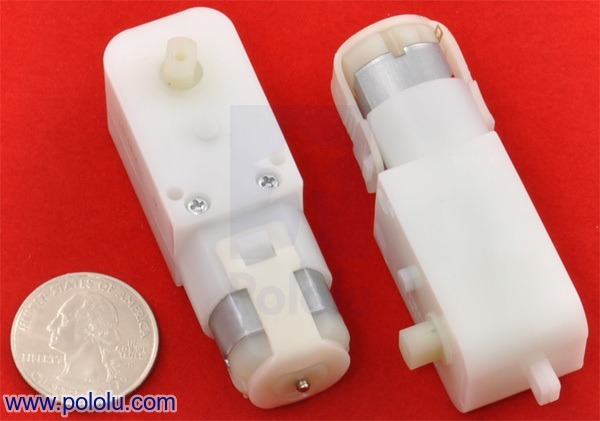
\includegraphics[height=5cm]{img/motores}
  \vspace{-0.3cm}
  \caption{Motores SolarBotics}
  \label{fig:motores}
\end{minipage}\hfill
\begin{minipage}{0.45\textwidth}
  \centering
  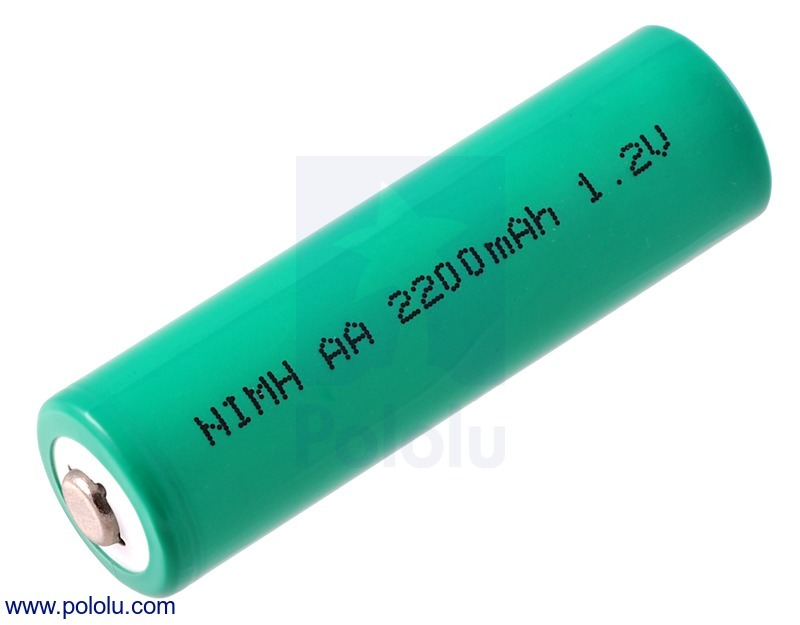
\includegraphics[height=5cm]{img/pila}
  \vspace{-0.3cm}
  \caption{Baterías de Litio - Ion}
  \label{fig:pilas}
\end{minipage}
\end{figure}

El tamaño del robot se ajusta a las dimensiones establecidas en los reglamentos de 10 cm x 10 cm.
La estructura mecánica se compone de 2 PCB unidos por 4 tornillos pasantes que los unen entre sí.
Entre los dos PCB se encuentran los motores (figura \ref{fig:motores})
Solarbotics\footnote{https://www.pololu.com/product/1121} con reducción 120:1 y 
dos baterías\footnote{https://www.pololu.com/product/1003} de Litio-Ion de $3.7$ V cada una, dando lugar utilizando una alimentación de $7.4$ V (figura \ref{fig:pilas}).
Utiliza ruedas de 70 mm de Solarbotics\footnote{https://www.pololu.com/product/184} (figura \ref{fig:ruedas}), 
con llantas de silicona de mayor adherencia \footnote{https://www.pololu.com/product/694} (figura \ref{fig:sticky}).

\begin{figure}
\centering
\begin{minipage}{0.45\textwidth}
  \centering
  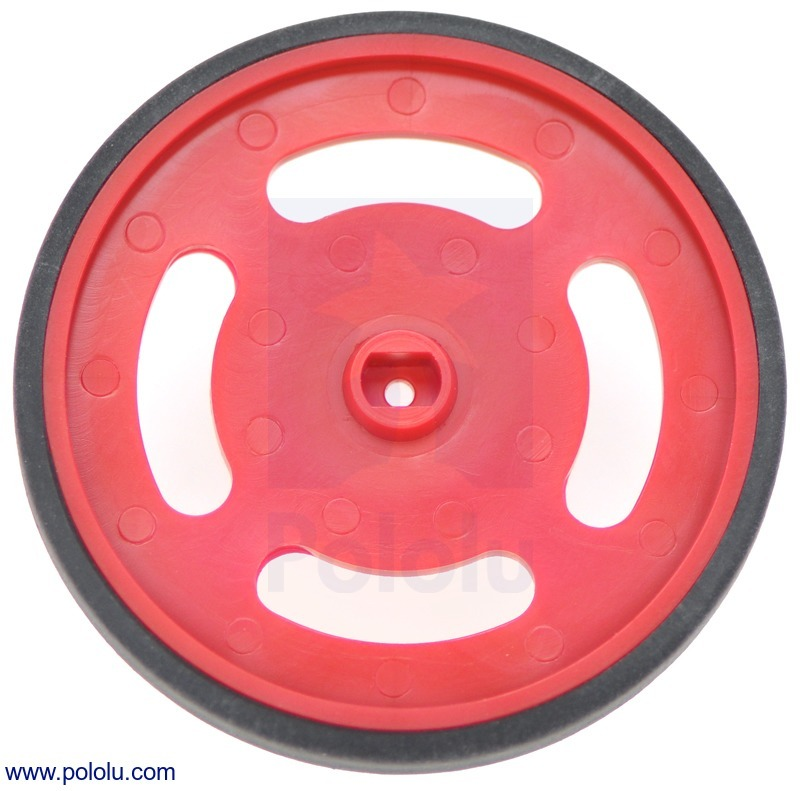
\includegraphics[height=4cm]{img/wheel}
  \vspace{-0.3cm}
  \caption{Ruedas Solarbotic 70 mm}
  \label{fig:ruedas}
\end{minipage}\hfill
\begin{minipage}{0.45\textwidth}
  \centering
  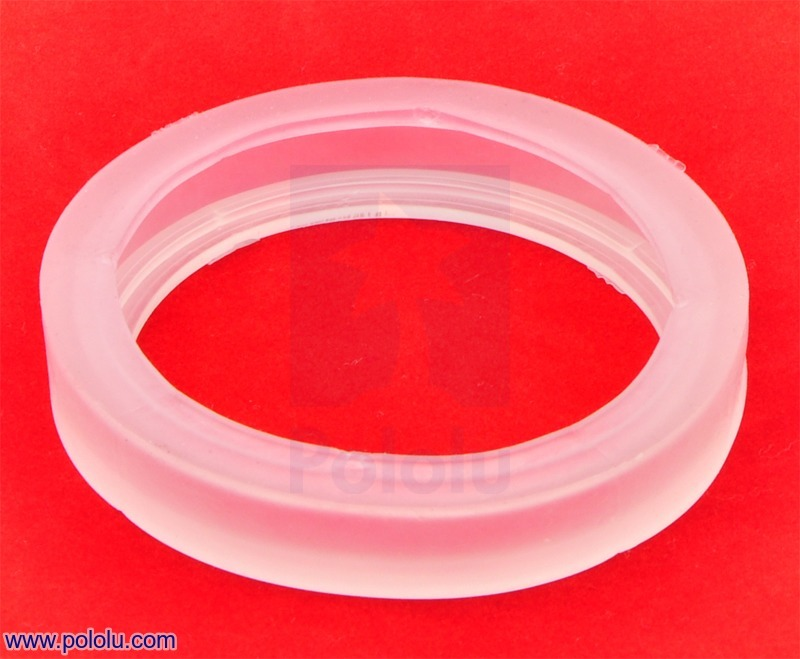
\includegraphics[height=5cm]{img/sticky}
  \vspace{-0.3cm}
  \caption{Goma de silicona de mayor adherencia}
  \label{fig:sticky}
\end{minipage}
\end{figure}

Se agregaron pilas en desuso para aumentar el peso del robot hasta alcanzar 500 g, que es el límite de la categoría. 

\section{Electrónica}

En la figura \ref{fig:sensores} se encuentra el circuito esquemático del PCB
inferior, que contiene los 4 sensores infrarrojos CNY70 que permiten detectar el
borde del tatami.

\begin{figure}[h!]
  \begin{center}
    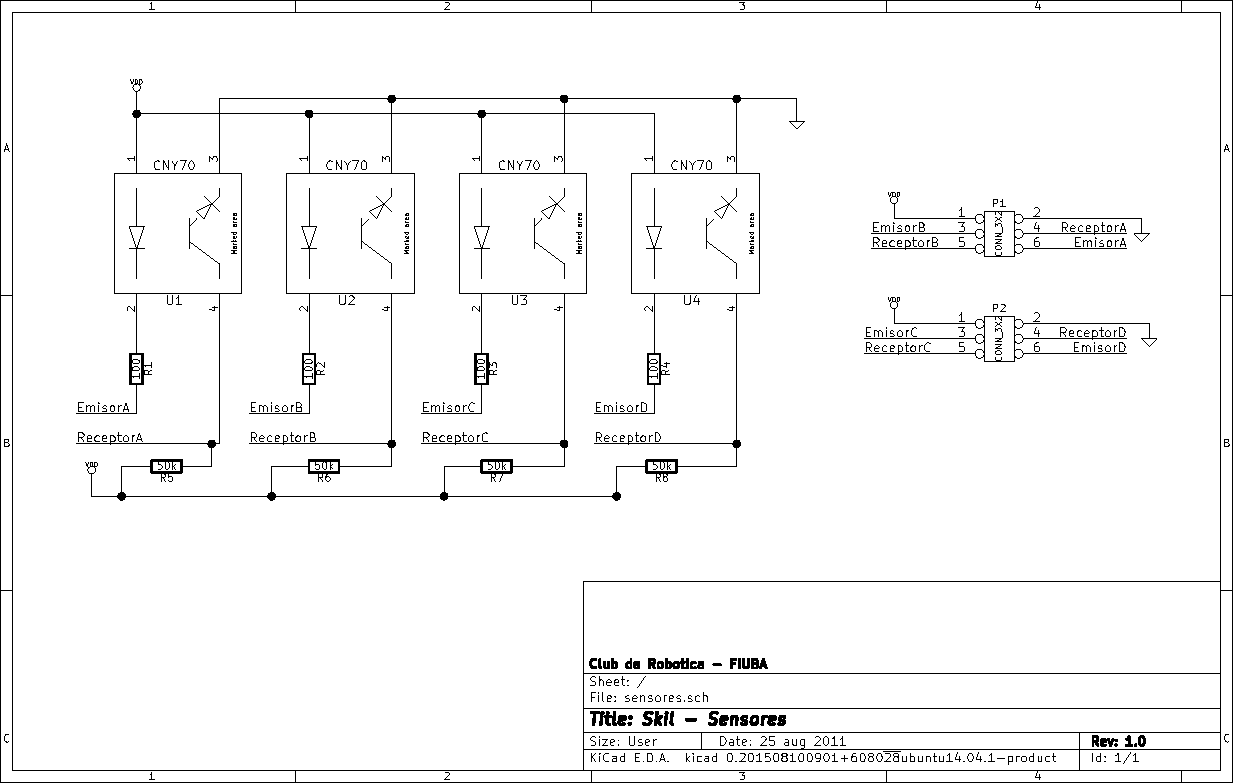
\includegraphics[width=0.9\textwidth]{img/sensores}
  \end{center}
  \vspace{-0.8cm}
  \caption{Circuito esqumático del PCB inferior}
  \label{fig:sensores}
\end{figure}

En la figura \ref{fig:mainboard} se encuentra el circuito esquemático del PCB
de la placa principal.
El circuito incluye el microcontrolador
ATmega88PA\footnote{http://www.atmel.com/devices/atmega88pa.aspx}, el
controlador de los motores, puente-H
DRV8833\footnote{http://www.ti.com/product/drv8833} y el emisor y receptor
infrarrojo que permite la detección del oponente.
Este circuito contemplaba la posibilidad de incluir un kit de desarrollo mBed\footnote{www.mbed.org}, aunque nunca se llevó a cabo.

\begin{figure}[h!]
  \begin{center}
    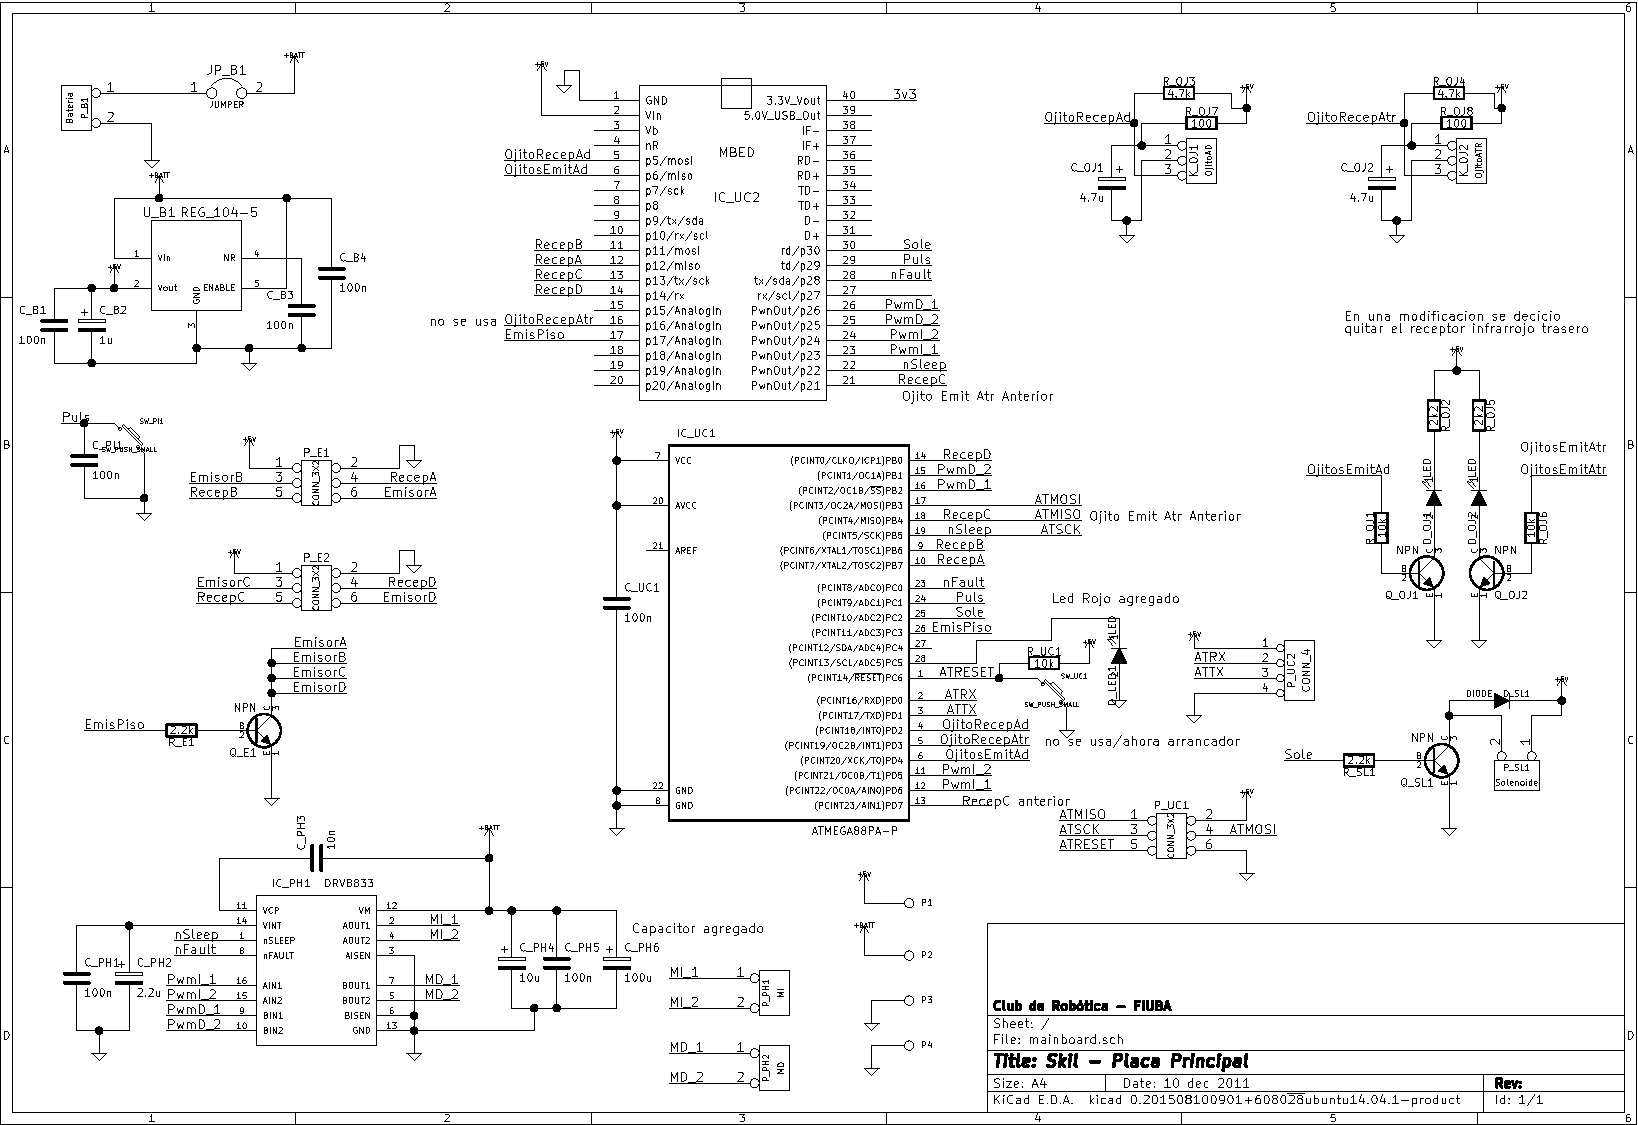
\includegraphics[height=17cm,angle=90]{img/mainboard}
  \end{center}
  \vspace{-0.8cm}
  \caption{Circuito esqumático del PCB superior}
  \label{fig:mainboard}
\end{figure}


\clearpage

\section{Código Fuente}

Se incluye el código fuente del programa principal. Todo el código fuente se puede encontrar en la página del proyecto

\url{http://labi.fi.uba.ar/chiliproject/projects/skil}

{
\footnotesize

\lstinputlisting{../src/atmega88/skil.c}
}

\end{document}

